\documentclass[11pt]{article}

    \usepackage[breakable]{tcolorbox}
    \usepackage{parskip} % Stop auto-indenting (to mimic markdown behaviour)
    
    \usepackage{iftex}
    \ifPDFTeX
    	\usepackage[T1]{fontenc}
    	\usepackage{mathpazo}
    \else
    	\usepackage{fontspec}
    \fi

    % Basic figure setup, for now with no caption control since it's done
    % automatically by Pandoc (which extracts ![](path) syntax from Markdown).
    \usepackage{graphicx}
    % Maintain compatibility with old templates. Remove in nbconvert 6.0
    \let\Oldincludegraphics\includegraphics
    % Ensure that by default, figures have no caption (until we provide a
    % proper Figure object with a Caption API and a way to capture that
    % in the conversion process - todo).
    \usepackage{caption}
    \DeclareCaptionFormat{nocaption}{}
    \captionsetup{format=nocaption,aboveskip=0pt,belowskip=0pt}

    \usepackage{float}
    \floatplacement{figure}{H} % forces figures to be placed at the correct location
    \usepackage{xcolor} % Allow colors to be defined
    \usepackage{enumerate} % Needed for markdown enumerations to work
    \usepackage{geometry} % Used to adjust the document margins
    \usepackage{amsmath} % Equations
    \usepackage{amssymb} % Equations
    \usepackage{textcomp} % defines textquotesingle
    % Hack from http://tex.stackexchange.com/a/47451/13684:
    \AtBeginDocument{%
        \def\PYZsq{\textquotesingle}% Upright quotes in Pygmentized code
    }
    \usepackage{upquote} % Upright quotes for verbatim code
    \usepackage{eurosym} % defines \euro
    \usepackage[mathletters]{ucs} % Extended unicode (utf-8) support
    \usepackage{fancyvrb} % verbatim replacement that allows latex
    \usepackage{grffile} % extends the file name processing of package graphics 
                         % to support a larger range
    \makeatletter % fix for old versions of grffile with XeLaTeX
    \@ifpackagelater{grffile}{2019/11/01}
    {
      % Do nothing on new versions
    }
    {
      \def\Gread@@xetex#1{%
        \IfFileExists{"\Gin@base".bb}%
        {\Gread@eps{\Gin@base.bb}}%
        {\Gread@@xetex@aux#1}%
      }
    }
    \makeatother
    \usepackage[Export]{adjustbox} % Used to constrain images to a maximum size
    \adjustboxset{max size={0.9\linewidth}{0.9\paperheight}}

    % The hyperref package gives us a pdf with properly built
    % internal navigation ('pdf bookmarks' for the table of contents,
    % internal cross-reference links, web links for URLs, etc.)
    \usepackage{hyperref}
    % The default LaTeX title has an obnoxious amount of whitespace. By default,
    % titling removes some of it. It also provides customization options.
    \usepackage{titling}
    \usepackage{longtable} % longtable support required by pandoc >1.10
    \usepackage{booktabs}  % table support for pandoc > 1.12.2
    \usepackage[inline]{enumitem} % IRkernel/repr support (it uses the enumerate* environment)
    \usepackage[normalem]{ulem} % ulem is needed to support strikethroughs (\sout)
                                % normalem makes italics be italics, not underlines
    \usepackage{mathrsfs}
    

    
    % Colors for the hyperref package
    \definecolor{urlcolor}{rgb}{0,.145,.698}
    \definecolor{linkcolor}{rgb}{.71,0.21,0.01}
    \definecolor{citecolor}{rgb}{.12,.54,.11}

    % ANSI colors
    \definecolor{ansi-black}{HTML}{3E424D}
    \definecolor{ansi-black-intense}{HTML}{282C36}
    \definecolor{ansi-red}{HTML}{E75C58}
    \definecolor{ansi-red-intense}{HTML}{B22B31}
    \definecolor{ansi-green}{HTML}{00A250}
    \definecolor{ansi-green-intense}{HTML}{007427}
    \definecolor{ansi-yellow}{HTML}{DDB62B}
    \definecolor{ansi-yellow-intense}{HTML}{B27D12}
    \definecolor{ansi-blue}{HTML}{208FFB}
    \definecolor{ansi-blue-intense}{HTML}{0065CA}
    \definecolor{ansi-magenta}{HTML}{D160C4}
    \definecolor{ansi-magenta-intense}{HTML}{A03196}
    \definecolor{ansi-cyan}{HTML}{60C6C8}
    \definecolor{ansi-cyan-intense}{HTML}{258F8F}
    \definecolor{ansi-white}{HTML}{C5C1B4}
    \definecolor{ansi-white-intense}{HTML}{A1A6B2}
    \definecolor{ansi-default-inverse-fg}{HTML}{FFFFFF}
    \definecolor{ansi-default-inverse-bg}{HTML}{000000}

    % common color for the border for error outputs.
    \definecolor{outerrorbackground}{HTML}{FFDFDF}

    % commands and environments needed by pandoc snippets
    % extracted from the output of `pandoc -s`
    \providecommand{\tightlist}{%
      \setlength{\itemsep}{0pt}\setlength{\parskip}{0pt}}
    \DefineVerbatimEnvironment{Highlighting}{Verbatim}{commandchars=\\\{\}}
    % Add ',fontsize=\small' for more characters per line
    \newenvironment{Shaded}{}{}
    \newcommand{\KeywordTok}[1]{\textcolor[rgb]{0.00,0.44,0.13}{\textbf{{#1}}}}
    \newcommand{\DataTypeTok}[1]{\textcolor[rgb]{0.56,0.13,0.00}{{#1}}}
    \newcommand{\DecValTok}[1]{\textcolor[rgb]{0.25,0.63,0.44}{{#1}}}
    \newcommand{\BaseNTok}[1]{\textcolor[rgb]{0.25,0.63,0.44}{{#1}}}
    \newcommand{\FloatTok}[1]{\textcolor[rgb]{0.25,0.63,0.44}{{#1}}}
    \newcommand{\CharTok}[1]{\textcolor[rgb]{0.25,0.44,0.63}{{#1}}}
    \newcommand{\StringTok}[1]{\textcolor[rgb]{0.25,0.44,0.63}{{#1}}}
    \newcommand{\CommentTok}[1]{\textcolor[rgb]{0.38,0.63,0.69}{\textit{{#1}}}}
    \newcommand{\OtherTok}[1]{\textcolor[rgb]{0.00,0.44,0.13}{{#1}}}
    \newcommand{\AlertTok}[1]{\textcolor[rgb]{1.00,0.00,0.00}{\textbf{{#1}}}}
    \newcommand{\FunctionTok}[1]{\textcolor[rgb]{0.02,0.16,0.49}{{#1}}}
    \newcommand{\RegionMarkerTok}[1]{{#1}}
    \newcommand{\ErrorTok}[1]{\textcolor[rgb]{1.00,0.00,0.00}{\textbf{{#1}}}}
    \newcommand{\NormalTok}[1]{{#1}}
    
    % Additional commands for more recent versions of Pandoc
    \newcommand{\ConstantTok}[1]{\textcolor[rgb]{0.53,0.00,0.00}{{#1}}}
    \newcommand{\SpecialCharTok}[1]{\textcolor[rgb]{0.25,0.44,0.63}{{#1}}}
    \newcommand{\VerbatimStringTok}[1]{\textcolor[rgb]{0.25,0.44,0.63}{{#1}}}
    \newcommand{\SpecialStringTok}[1]{\textcolor[rgb]{0.73,0.40,0.53}{{#1}}}
    \newcommand{\ImportTok}[1]{{#1}}
    \newcommand{\DocumentationTok}[1]{\textcolor[rgb]{0.73,0.13,0.13}{\textit{{#1}}}}
    \newcommand{\AnnotationTok}[1]{\textcolor[rgb]{0.38,0.63,0.69}{\textbf{\textit{{#1}}}}}
    \newcommand{\CommentVarTok}[1]{\textcolor[rgb]{0.38,0.63,0.69}{\textbf{\textit{{#1}}}}}
    \newcommand{\VariableTok}[1]{\textcolor[rgb]{0.10,0.09,0.49}{{#1}}}
    \newcommand{\ControlFlowTok}[1]{\textcolor[rgb]{0.00,0.44,0.13}{\textbf{{#1}}}}
    \newcommand{\OperatorTok}[1]{\textcolor[rgb]{0.40,0.40,0.40}{{#1}}}
    \newcommand{\BuiltInTok}[1]{{#1}}
    \newcommand{\ExtensionTok}[1]{{#1}}
    \newcommand{\PreprocessorTok}[1]{\textcolor[rgb]{0.74,0.48,0.00}{{#1}}}
    \newcommand{\AttributeTok}[1]{\textcolor[rgb]{0.49,0.56,0.16}{{#1}}}
    \newcommand{\InformationTok}[1]{\textcolor[rgb]{0.38,0.63,0.69}{\textbf{\textit{{#1}}}}}
    \newcommand{\WarningTok}[1]{\textcolor[rgb]{0.38,0.63,0.69}{\textbf{\textit{{#1}}}}}
    
    
    % Define a nice break command that doesn't care if a line doesn't already
    % exist.
    \def\br{\hspace*{\fill} \\* }
    % Math Jax compatibility definitions
    \def\gt{>}
    \def\lt{<}
    \let\Oldtex\TeX
    \let\Oldlatex\LaTeX
    \renewcommand{\TeX}{\textrm{\Oldtex}}
    \renewcommand{\LaTeX}{\textrm{\Oldlatex}}
    % Document parameters
    % Document title
    \title{Ballistic Pendulum Lab}
    \author{Isaac Robinson}
    
    
    
    
    
% Pygments definitions
\makeatletter
\def\PY@reset{\let\PY@it=\relax \let\PY@bf=\relax%
    \let\PY@ul=\relax \let\PY@tc=\relax%
    \let\PY@bc=\relax \let\PY@ff=\relax}
\def\PY@tok#1{\csname PY@tok@#1\endcsname}
\def\PY@toks#1+{\ifx\relax#1\empty\else%
    \PY@tok{#1}\expandafter\PY@toks\fi}
\def\PY@do#1{\PY@bc{\PY@tc{\PY@ul{%
    \PY@it{\PY@bf{\PY@ff{#1}}}}}}}
\def\PY#1#2{\PY@reset\PY@toks#1+\relax+\PY@do{#2}}

\expandafter\def\csname PY@tok@w\endcsname{\def\PY@tc##1{\textcolor[rgb]{0.73,0.73,0.73}{##1}}}
\expandafter\def\csname PY@tok@c\endcsname{\let\PY@it=\textit\def\PY@tc##1{\textcolor[rgb]{0.25,0.50,0.50}{##1}}}
\expandafter\def\csname PY@tok@cp\endcsname{\def\PY@tc##1{\textcolor[rgb]{0.74,0.48,0.00}{##1}}}
\expandafter\def\csname PY@tok@k\endcsname{\let\PY@bf=\textbf\def\PY@tc##1{\textcolor[rgb]{0.00,0.50,0.00}{##1}}}
\expandafter\def\csname PY@tok@kp\endcsname{\def\PY@tc##1{\textcolor[rgb]{0.00,0.50,0.00}{##1}}}
\expandafter\def\csname PY@tok@kt\endcsname{\def\PY@tc##1{\textcolor[rgb]{0.69,0.00,0.25}{##1}}}
\expandafter\def\csname PY@tok@o\endcsname{\def\PY@tc##1{\textcolor[rgb]{0.40,0.40,0.40}{##1}}}
\expandafter\def\csname PY@tok@ow\endcsname{\let\PY@bf=\textbf\def\PY@tc##1{\textcolor[rgb]{0.67,0.13,1.00}{##1}}}
\expandafter\def\csname PY@tok@nb\endcsname{\def\PY@tc##1{\textcolor[rgb]{0.00,0.50,0.00}{##1}}}
\expandafter\def\csname PY@tok@nf\endcsname{\def\PY@tc##1{\textcolor[rgb]{0.00,0.00,1.00}{##1}}}
\expandafter\def\csname PY@tok@nc\endcsname{\let\PY@bf=\textbf\def\PY@tc##1{\textcolor[rgb]{0.00,0.00,1.00}{##1}}}
\expandafter\def\csname PY@tok@nn\endcsname{\let\PY@bf=\textbf\def\PY@tc##1{\textcolor[rgb]{0.00,0.00,1.00}{##1}}}
\expandafter\def\csname PY@tok@ne\endcsname{\let\PY@bf=\textbf\def\PY@tc##1{\textcolor[rgb]{0.82,0.25,0.23}{##1}}}
\expandafter\def\csname PY@tok@nv\endcsname{\def\PY@tc##1{\textcolor[rgb]{0.10,0.09,0.49}{##1}}}
\expandafter\def\csname PY@tok@no\endcsname{\def\PY@tc##1{\textcolor[rgb]{0.53,0.00,0.00}{##1}}}
\expandafter\def\csname PY@tok@nl\endcsname{\def\PY@tc##1{\textcolor[rgb]{0.63,0.63,0.00}{##1}}}
\expandafter\def\csname PY@tok@ni\endcsname{\let\PY@bf=\textbf\def\PY@tc##1{\textcolor[rgb]{0.60,0.60,0.60}{##1}}}
\expandafter\def\csname PY@tok@na\endcsname{\def\PY@tc##1{\textcolor[rgb]{0.49,0.56,0.16}{##1}}}
\expandafter\def\csname PY@tok@nt\endcsname{\let\PY@bf=\textbf\def\PY@tc##1{\textcolor[rgb]{0.00,0.50,0.00}{##1}}}
\expandafter\def\csname PY@tok@nd\endcsname{\def\PY@tc##1{\textcolor[rgb]{0.67,0.13,1.00}{##1}}}
\expandafter\def\csname PY@tok@s\endcsname{\def\PY@tc##1{\textcolor[rgb]{0.73,0.13,0.13}{##1}}}
\expandafter\def\csname PY@tok@sd\endcsname{\let\PY@it=\textit\def\PY@tc##1{\textcolor[rgb]{0.73,0.13,0.13}{##1}}}
\expandafter\def\csname PY@tok@si\endcsname{\let\PY@bf=\textbf\def\PY@tc##1{\textcolor[rgb]{0.73,0.40,0.53}{##1}}}
\expandafter\def\csname PY@tok@se\endcsname{\let\PY@bf=\textbf\def\PY@tc##1{\textcolor[rgb]{0.73,0.40,0.13}{##1}}}
\expandafter\def\csname PY@tok@sr\endcsname{\def\PY@tc##1{\textcolor[rgb]{0.73,0.40,0.53}{##1}}}
\expandafter\def\csname PY@tok@ss\endcsname{\def\PY@tc##1{\textcolor[rgb]{0.10,0.09,0.49}{##1}}}
\expandafter\def\csname PY@tok@sx\endcsname{\def\PY@tc##1{\textcolor[rgb]{0.00,0.50,0.00}{##1}}}
\expandafter\def\csname PY@tok@m\endcsname{\def\PY@tc##1{\textcolor[rgb]{0.40,0.40,0.40}{##1}}}
\expandafter\def\csname PY@tok@gh\endcsname{\let\PY@bf=\textbf\def\PY@tc##1{\textcolor[rgb]{0.00,0.00,0.50}{##1}}}
\expandafter\def\csname PY@tok@gu\endcsname{\let\PY@bf=\textbf\def\PY@tc##1{\textcolor[rgb]{0.50,0.00,0.50}{##1}}}
\expandafter\def\csname PY@tok@gd\endcsname{\def\PY@tc##1{\textcolor[rgb]{0.63,0.00,0.00}{##1}}}
\expandafter\def\csname PY@tok@gi\endcsname{\def\PY@tc##1{\textcolor[rgb]{0.00,0.63,0.00}{##1}}}
\expandafter\def\csname PY@tok@gr\endcsname{\def\PY@tc##1{\textcolor[rgb]{1.00,0.00,0.00}{##1}}}
\expandafter\def\csname PY@tok@ge\endcsname{\let\PY@it=\textit}
\expandafter\def\csname PY@tok@gs\endcsname{\let\PY@bf=\textbf}
\expandafter\def\csname PY@tok@gp\endcsname{\let\PY@bf=\textbf\def\PY@tc##1{\textcolor[rgb]{0.00,0.00,0.50}{##1}}}
\expandafter\def\csname PY@tok@go\endcsname{\def\PY@tc##1{\textcolor[rgb]{0.53,0.53,0.53}{##1}}}
\expandafter\def\csname PY@tok@gt\endcsname{\def\PY@tc##1{\textcolor[rgb]{0.00,0.27,0.87}{##1}}}
\expandafter\def\csname PY@tok@err\endcsname{\def\PY@bc##1{\setlength{\fboxsep}{0pt}\fcolorbox[rgb]{1.00,0.00,0.00}{1,1,1}{\strut ##1}}}
\expandafter\def\csname PY@tok@kc\endcsname{\let\PY@bf=\textbf\def\PY@tc##1{\textcolor[rgb]{0.00,0.50,0.00}{##1}}}
\expandafter\def\csname PY@tok@kd\endcsname{\let\PY@bf=\textbf\def\PY@tc##1{\textcolor[rgb]{0.00,0.50,0.00}{##1}}}
\expandafter\def\csname PY@tok@kn\endcsname{\let\PY@bf=\textbf\def\PY@tc##1{\textcolor[rgb]{0.00,0.50,0.00}{##1}}}
\expandafter\def\csname PY@tok@kr\endcsname{\let\PY@bf=\textbf\def\PY@tc##1{\textcolor[rgb]{0.00,0.50,0.00}{##1}}}
\expandafter\def\csname PY@tok@bp\endcsname{\def\PY@tc##1{\textcolor[rgb]{0.00,0.50,0.00}{##1}}}
\expandafter\def\csname PY@tok@fm\endcsname{\def\PY@tc##1{\textcolor[rgb]{0.00,0.00,1.00}{##1}}}
\expandafter\def\csname PY@tok@vc\endcsname{\def\PY@tc##1{\textcolor[rgb]{0.10,0.09,0.49}{##1}}}
\expandafter\def\csname PY@tok@vg\endcsname{\def\PY@tc##1{\textcolor[rgb]{0.10,0.09,0.49}{##1}}}
\expandafter\def\csname PY@tok@vi\endcsname{\def\PY@tc##1{\textcolor[rgb]{0.10,0.09,0.49}{##1}}}
\expandafter\def\csname PY@tok@vm\endcsname{\def\PY@tc##1{\textcolor[rgb]{0.10,0.09,0.49}{##1}}}
\expandafter\def\csname PY@tok@sa\endcsname{\def\PY@tc##1{\textcolor[rgb]{0.73,0.13,0.13}{##1}}}
\expandafter\def\csname PY@tok@sb\endcsname{\def\PY@tc##1{\textcolor[rgb]{0.73,0.13,0.13}{##1}}}
\expandafter\def\csname PY@tok@sc\endcsname{\def\PY@tc##1{\textcolor[rgb]{0.73,0.13,0.13}{##1}}}
\expandafter\def\csname PY@tok@dl\endcsname{\def\PY@tc##1{\textcolor[rgb]{0.73,0.13,0.13}{##1}}}
\expandafter\def\csname PY@tok@s2\endcsname{\def\PY@tc##1{\textcolor[rgb]{0.73,0.13,0.13}{##1}}}
\expandafter\def\csname PY@tok@sh\endcsname{\def\PY@tc##1{\textcolor[rgb]{0.73,0.13,0.13}{##1}}}
\expandafter\def\csname PY@tok@s1\endcsname{\def\PY@tc##1{\textcolor[rgb]{0.73,0.13,0.13}{##1}}}
\expandafter\def\csname PY@tok@mb\endcsname{\def\PY@tc##1{\textcolor[rgb]{0.40,0.40,0.40}{##1}}}
\expandafter\def\csname PY@tok@mf\endcsname{\def\PY@tc##1{\textcolor[rgb]{0.40,0.40,0.40}{##1}}}
\expandafter\def\csname PY@tok@mh\endcsname{\def\PY@tc##1{\textcolor[rgb]{0.40,0.40,0.40}{##1}}}
\expandafter\def\csname PY@tok@mi\endcsname{\def\PY@tc##1{\textcolor[rgb]{0.40,0.40,0.40}{##1}}}
\expandafter\def\csname PY@tok@il\endcsname{\def\PY@tc##1{\textcolor[rgb]{0.40,0.40,0.40}{##1}}}
\expandafter\def\csname PY@tok@mo\endcsname{\def\PY@tc##1{\textcolor[rgb]{0.40,0.40,0.40}{##1}}}
\expandafter\def\csname PY@tok@ch\endcsname{\let\PY@it=\textit\def\PY@tc##1{\textcolor[rgb]{0.25,0.50,0.50}{##1}}}
\expandafter\def\csname PY@tok@cm\endcsname{\let\PY@it=\textit\def\PY@tc##1{\textcolor[rgb]{0.25,0.50,0.50}{##1}}}
\expandafter\def\csname PY@tok@cpf\endcsname{\let\PY@it=\textit\def\PY@tc##1{\textcolor[rgb]{0.25,0.50,0.50}{##1}}}
\expandafter\def\csname PY@tok@c1\endcsname{\let\PY@it=\textit\def\PY@tc##1{\textcolor[rgb]{0.25,0.50,0.50}{##1}}}
\expandafter\def\csname PY@tok@cs\endcsname{\let\PY@it=\textit\def\PY@tc##1{\textcolor[rgb]{0.25,0.50,0.50}{##1}}}

\def\PYZbs{\char`\\}
\def\PYZus{\char`\_}
\def\PYZob{\char`\{}
\def\PYZcb{\char`\}}
\def\PYZca{\char`\^}
\def\PYZam{\char`\&}
\def\PYZlt{\char`\<}
\def\PYZgt{\char`\>}
\def\PYZsh{\char`\#}
\def\PYZpc{\char`\%}
\def\PYZdl{\char`\$}
\def\PYZhy{\char`\-}
\def\PYZsq{\char`\'}
\def\PYZdq{\char`\"}
\def\PYZti{\char`\~}
% for compatibility with earlier versions
\def\PYZat{@}
\def\PYZlb{[}
\def\PYZrb{]}
\makeatother


    % For linebreaks inside Verbatim environment from package fancyvrb. 
    \makeatletter
        \newbox\Wrappedcontinuationbox 
        \newbox\Wrappedvisiblespacebox 
        \newcommand*\Wrappedvisiblespace {\textcolor{red}{\textvisiblespace}} 
        \newcommand*\Wrappedcontinuationsymbol {\textcolor{red}{\llap{\tiny$\m@th\hookrightarrow$}}} 
        \newcommand*\Wrappedcontinuationindent {3ex } 
        \newcommand*\Wrappedafterbreak {\kern\Wrappedcontinuationindent\copy\Wrappedcontinuationbox} 
        % Take advantage of the already applied Pygments mark-up to insert 
        % potential linebreaks for TeX processing. 
        %        {, <, #, %, $, ' and ": go to next line. 
        %        _, }, ^, &, >, - and ~: stay at end of broken line. 
        % Use of \textquotesingle for straight quote. 
        \newcommand*\Wrappedbreaksatspecials {% 
            \def\PYGZus{\discretionary{\char`\_}{\Wrappedafterbreak}{\char`\_}}% 
            \def\PYGZob{\discretionary{}{\Wrappedafterbreak\char`\{}{\char`\{}}% 
            \def\PYGZcb{\discretionary{\char`\}}{\Wrappedafterbreak}{\char`\}}}% 
            \def\PYGZca{\discretionary{\char`\^}{\Wrappedafterbreak}{\char`\^}}% 
            \def\PYGZam{\discretionary{\char`\&}{\Wrappedafterbreak}{\char`\&}}% 
            \def\PYGZlt{\discretionary{}{\Wrappedafterbreak\char`\<}{\char`\<}}% 
            \def\PYGZgt{\discretionary{\char`\>}{\Wrappedafterbreak}{\char`\>}}% 
            \def\PYGZsh{\discretionary{}{\Wrappedafterbreak\char`\#}{\char`\#}}% 
            \def\PYGZpc{\discretionary{}{\Wrappedafterbreak\char`\%}{\char`\%}}% 
            \def\PYGZdl{\discretionary{}{\Wrappedafterbreak\char`\$}{\char`\$}}% 
            \def\PYGZhy{\discretionary{\char`\-}{\Wrappedafterbreak}{\char`\-}}% 
            \def\PYGZsq{\discretionary{}{\Wrappedafterbreak\textquotesingle}{\textquotesingle}}% 
            \def\PYGZdq{\discretionary{}{\Wrappedafterbreak\char`\"}{\char`\"}}% 
            \def\PYGZti{\discretionary{\char`\~}{\Wrappedafterbreak}{\char`\~}}% 
        } 
        % Some characters . , ; ? ! / are not pygmentized. 
        % This macro makes them "active" and they will insert potential linebreaks 
        \newcommand*\Wrappedbreaksatpunct {% 
            \lccode`\~`\.\lowercase{\def~}{\discretionary{\hbox{\char`\.}}{\Wrappedafterbreak}{\hbox{\char`\.}}}% 
            \lccode`\~`\,\lowercase{\def~}{\discretionary{\hbox{\char`\,}}{\Wrappedafterbreak}{\hbox{\char`\,}}}% 
            \lccode`\~`\;\lowercase{\def~}{\discretionary{\hbox{\char`\;}}{\Wrappedafterbreak}{\hbox{\char`\;}}}% 
            \lccode`\~`\:\lowercase{\def~}{\discretionary{\hbox{\char`\:}}{\Wrappedafterbreak}{\hbox{\char`\:}}}% 
            \lccode`\~`\?\lowercase{\def~}{\discretionary{\hbox{\char`\?}}{\Wrappedafterbreak}{\hbox{\char`\?}}}% 
            \lccode`\~`\!\lowercase{\def~}{\discretionary{\hbox{\char`\!}}{\Wrappedafterbreak}{\hbox{\char`\!}}}% 
            \lccode`\~`\/\lowercase{\def~}{\discretionary{\hbox{\char`\/}}{\Wrappedafterbreak}{\hbox{\char`\/}}}% 
            \catcode`\.\active
            \catcode`\,\active 
            \catcode`\;\active
            \catcode`\:\active
            \catcode`\?\active
            \catcode`\!\active
            \catcode`\/\active 
            \lccode`\~`\~ 	
        }
    \makeatother

    \let\OriginalVerbatim=\Verbatim
    \makeatletter
    \renewcommand{\Verbatim}[1][1]{%
        %\parskip\z@skip
        \sbox\Wrappedcontinuationbox {\Wrappedcontinuationsymbol}%
        \sbox\Wrappedvisiblespacebox {\FV@SetupFont\Wrappedvisiblespace}%
        \def\FancyVerbFormatLine ##1{\hsize\linewidth
            \vtop{\raggedright\hyphenpenalty\z@\exhyphenpenalty\z@
                \doublehyphendemerits\z@\finalhyphendemerits\z@
                \strut ##1\strut}%
        }%
        % If the linebreak is at a space, the latter will be displayed as visible
        % space at end of first line, and a continuation symbol starts next line.
        % Stretch/shrink are however usually zero for typewriter font.
        \def\FV@Space {%
            \nobreak\hskip\z@ plus\fontdimen3\font minus\fontdimen4\font
            \discretionary{\copy\Wrappedvisiblespacebox}{\Wrappedafterbreak}
            {\kern\fontdimen2\font}%
        }%
        
        % Allow breaks at special characters using \PYG... macros.
        \Wrappedbreaksatspecials
        % Breaks at punctuation characters . , ; ? ! and / need catcode=\active 	
        \OriginalVerbatim[#1,codes*=\Wrappedbreaksatpunct]%
    }
    \makeatother

    % Exact colors from NB
    \definecolor{incolor}{HTML}{303F9F}
    \definecolor{outcolor}{HTML}{D84315}
    \definecolor{cellborder}{HTML}{CFCFCF}
    \definecolor{cellbackground}{HTML}{F7F7F7}
    
    % prompt
    \makeatletter
    \newcommand{\boxspacing}{\kern\kvtcb@left@rule\kern\kvtcb@boxsep}
    \makeatother
    \newcommand{\prompt}[4]{
        {\ttfamily\llap{{\color{#2}[#3]:\hspace{3pt}#4}}\vspace{-\baselineskip}}
    }
    

    
    % Prevent overflowing lines due to hard-to-break entities
    \sloppy 
    % Setup hyperref package
    \hypersetup{
      breaklinks=true,  % so long urls are correctly broken across lines
      colorlinks=true,
      urlcolor=urlcolor,
      linkcolor=linkcolor,
      citecolor=citecolor,
      }
    % Slightly bigger margins than the latex defaults
    
    \geometry{verbose,tmargin=1in,bmargin=1in,lmargin=1in,rmargin=1in}
    
    

\begin{document}
    
    \maketitle
    
    

    
    \hypertarget{abstract}{%
\subsection*{\centering Abstract}\label{abstract}}

The goal of this experiment was to compare 2 computational physical
models to each other by computing the initial velocity of a projectile
using both methods and comparing the result to check for consistency.
The first method launched the projectile into a pendulum and used the
conservation of energy and conservation of momentum laws to compute the
initial velocity from the max angle the pendulum reached, while the
second method used kinematics equations to find the initial velocity
from the projectile's launch height and distance traveled. The results
didn't equate, but it was concluded that this was likely due to
underestimating the error of certain values in parts 1 and 2 of the
experiment.

\hypertarget{introduction}{%
\subsection*{\centering Introduction}\label{introduction}}

In this lab, the initial velocity of a projectile was calculated using
two fundamental physical models, and the results were compared to see if
the models agree with each other. The two models that were used to
compute the ball's initial velocity in this experiment were the
conservation of energy laws and kinematics equations.

\hypertarget{method-1}{%
\subsubsection*{\centering Method 1}\label{method-1}}

First, the velocity of the projectile was calculated using the
conservation of momentum and the conservation of energy laws. To do
this, the projectile(a round metal ball) was launched into a pendulum,
which captured the ball. Then the max angle of the pendulum was taken as
it swung up, as shown in Figure 1. 
\begin{figure}
\begin{center}
 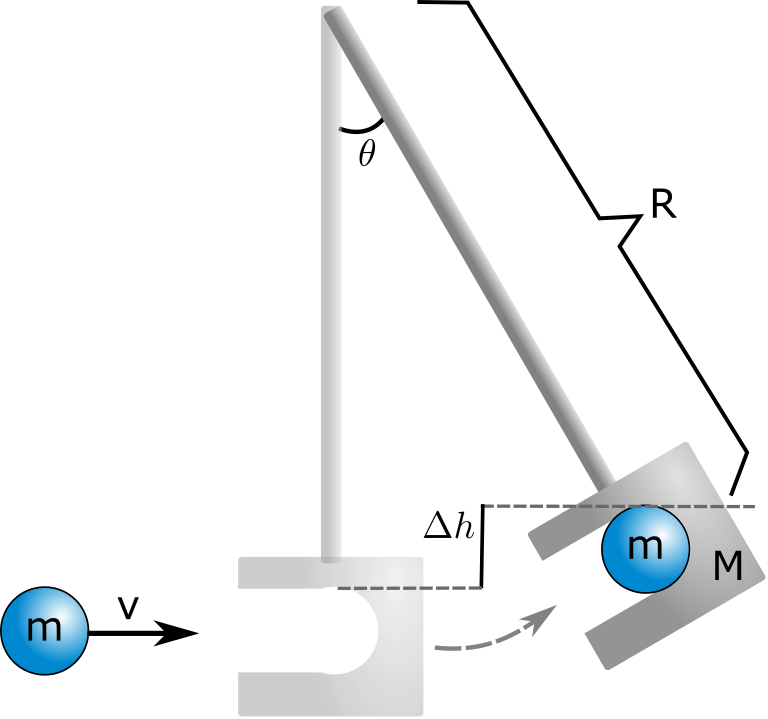
\includegraphics[scale=0.4]{Part1Diagram.png}
 
\textbf{Figure 1:} A ball in motion collides with a pendulum, causing it to swing up.
\end{center}
\end{figure}
The collision between the pendulum and the ball is inelastic, and
therefore the momentum before the collision must be maintained after the
collision. If the mass of the ball is defined as \(m\), the velocity of
the ball as \(v\), the mass of the pendulum as \(M\), and the velocity
of the pendulum and ball combined as \(V\), the relationship can be
defined as \(mv=(m + M)V\). Rearranging this formula provides a way to
solve for the original ball's velocity.

\begin{equation}
v = \frac {(m + M)V}{m}
\end{equation}

By further observation of the system, it can be seen that the energy of
the system is conserved, and is either stored in the form of kinetic or
gravitational potential energy. Immediately after the collision, all
energy is of kinetic form, and can be easily calculated using
\(KE = \frac{1}{2}(m + M)V^2\). When the pendulum reaches its maximum
height or angle, the pendulum stops for a split second. Therefore, all
energy is found in gravitational potential form and can be expressed as
\(PE=(m + M)g\Delta h\). Applying the conservation of energy law, it can
be assumed the initial kinetic energy is equal to the final potential
energy. This can be written as below, and rewritten to solve for the
velocity of the pendulum.

\[
\frac{1}{2}(m + M)V^2 = (m + M)g\Delta h
\]
\begin{equation}
V = \sqrt{2g \Delta h}
\end{equation}

It is possible to compute the height the pendulum lifts by the
application of trigonometric functions. The height is the difference
between the pendulum height and the final y component of the pendulum.
If the length of the pendulum bob is defined as \(R\), and the angle is
defined as \(\theta\), the change in the height of the pendulum can be
expressed as below.

\begin{equation}
\Delta h = R - R \cos(\theta) = R(1 - \cos(\theta))
\end{equation}

By combining equations \((1)\), \((2)\), and \((3)\), as shown above,
the initial velocity of the ball can be computed from the pendulum
height and angle using the formula shown below.

\begin{equation}
v = \frac {m + M}{m} \sqrt {2gR(1 - cos(\theta))}
\end{equation}

\hypertarget{method-2}{%
\subsubsection*{\centering Method 2}\label{method-2}}

For the second part, the velocity of the projectile was measured using
kinematics equations. To accomplish this, the ball was launched from a
table with a given height and the distance the ball traveled was
measured, as shown in figure 2. 
\begin{figure}
\begin{center}
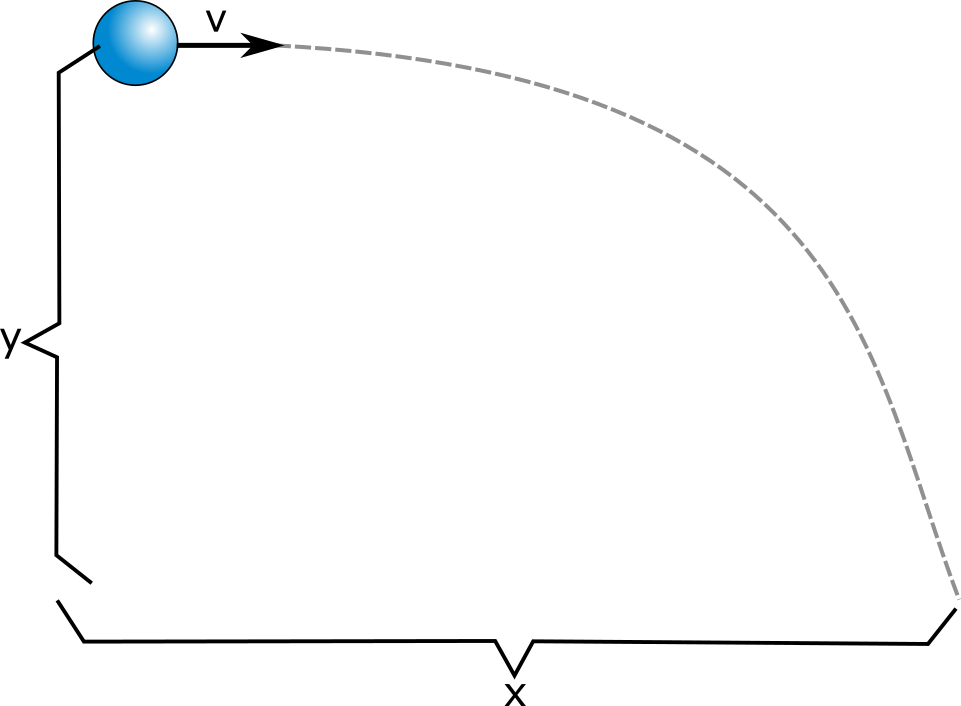
\includegraphics[scale=0.4]{Part2Diagram.png}

\textbf{Figure 2:} A trace of the path of a projectile launched with a constant velocity in the x-direction.
\end{center}
\end{figure}
Ignoring air resistance, given its impact on the system is minimal,
there is no acceleration in the x-direction. The only acceleration which
affects the system is the acceleration due to gravity, which only acts
on the y component of the motion. This system can be represented using 2
kinematic equations, namely \(\Delta x = v_i t\) and
\(\Delta y = \frac{1}{2}gt^2\), where \(\Delta x\) is the displacement
on the x-axis, \(\Delta y\) is the displacement on the y-axis, and
\(v_i\) is the initial velocity. Solving this system for \(v_i\) gives
us the formula below for computing the initial velocity.

\begin{equation}
v_i = \Delta x \sqrt{\frac {g}{2\Delta y}}
\end{equation}

\hypertarget{data}{%
\subsection*{\centering Data}\label{data}}

\hypertarget{method-1-1}{%
\subsubsection*{\centering Method 1}\label{method-1-1}}

For the first part of the experiment the length of the pendulum \(R\),
the mass of the pendulum \(M\), and the mass of the ball \(m\) were
needed. The length of the pendulum from the pivot point to the center of
mass was measured to be \(R=27.70 \pm 0.20\text{ }cm\). The center of
mass was determined by adjusting the pendulum until it balanced on a
thin metal pole. The mass of the pendulum was measured on a digital
scale to be \(M = 191.70 \pm 0.10\text{ }g\). The mass of the ball, also
measured on a digital scale, was determined to be
\(m = 65.50 \pm 0.10\text{ }g\). Once all preliminary measurements were
taken, the ball was launched into the pendulum 10 times, and the max
angle the pendulum reached was recorded. The resulting angles can be
seen in Table 1.

\begin{center}
\textbf{Table 1}

\begin{tabular}{rr}
\toprule
 Trial &  Theta $\theta^{\circ}$ \\
\midrule
     1 &                    45.0 \\
     2 &                    46.0 \\
     3 &                    45.5 \\
     4 &                    46.0 \\
     5 &                    46.0 \\
     6 &                    46.0 \\
     7 &                    46.0 \\
     8 &                    46.0 \\
     9 &                    46.0 \\
    10 &                    46.0 \\
\bottomrule
\end{tabular}
\end{center}

\hypertarget{method-2-1}{%
\subsubsection*{\centering Method 2}\label{method-2-1}}

For the second part of the experiment, the ball was launched onto a
piece of carbon paper placed on the ground, and the impact of the ball
would leave a mark in the regular piece of paper placed underneath the
ball. The distance from the edge of the paper to the table was measured
to be 193.70 cm, and the distance from the edge of the table to the
launcher was measured and recorded as 18.10 cm. Once these values were
calculated, the ball was launched 11 times, and the distance from the
edge of the paper to the ball impact was recorded. The resulting
measurements can be seen in Table 2.

\begin{center}
\textbf{Table 2}

\begin{tabular}{rr}
\toprule
 Trial &  Distance (cm) \\
\midrule
     1 &            6.0 \\
     2 &            6.5 \\
     3 &            7.0 \\
     4 &            7.2 \\
     5 &            7.3 \\
     6 &            8.5 \\
     7 &            8.8 \\
     8 &            9.2 \\
     9 &            9.8 \\
    10 &            9.0 \\
    11 &            8.6 \\
\bottomrule
\end{tabular}
\end{center}

\hypertarget{data-analysis-and-results}{%
\subsection*{\centering Data Analysis and Results}\label{data-analysis-and-results}}

\hypertarget{method-1-2}{%
\subsubsection*{\centering Method 1}\label{method-1-2}}

After the data was collected, the average maximum swing angle was
computed to be \(\theta_{avg} =0.80\text{ rad}\). Once the average angle
was computed, the average angle and the length of the pendulum were
substituted into equation \((4)\).

\begin{equation}
v = \frac {m + M}{m} \sqrt {2gR(1 - cos(\theta))} = \frac {m + M}{m} \sqrt {2gR(1 - cos(\theta_{avg}))}
\end{equation}
\[
v = 5.04 \text{ }\frac {m}{s}
\]

The uncertainty of the velocity still needed to be calculated. The
formula for uncertainty was found by applying the rules of error
propagation, specifically rule 4.

\begin{equation}
\delta v = v \sqrt{(\frac{\delta(m + M)}{m + M})^2 + (-\frac{\delta m}{m})^2 + (\frac{\delta R}{2R})^2
+ (\frac{\delta(1 - \cos(\theta))}{2(1 - \cos(\theta))})^2}
\end{equation}


The above formula has several other errors that need to be calculated.
To get \(\delta(m + M)\), we can apply error propagation rule 2, which
gives us \(\delta(m + M) = \sqrt{\delta m^2 + \delta M^2}\). The
uncertainty of \(m\) and \(M\) was \(0.10 \text{ }g\) and
\(0.10 \text{ }g\), respectively, as determined by the known uncertainty
of the measuring instruments used. Plugging \(m\) and \(M\) into the
formula above gave a result of \(0.14 \text{ }g\). To get
\(\delta(1 - \cos(\theta))\), every angle was run through
\(1 - \cos(\theta)\), and the standard deviation of all of these values
was taken and divided by the number of trials. This formula takes the
form below.

\begin{equation}
\delta(1 - \cos(\theta)) = \frac {\sigma}{\sqrt{n}} = \frac {\sigma(1 - \cos(\theta))}{\sqrt{n}}
\end{equation}

 Where the standard deviation is.
 
 \begin{equation}
\sigma(X)=\sqrt{\frac{1}{N-1}\sum_{i=1}^N(X_i - X_{avg})^2}
\end{equation}

Applying this formula results in
\(\delta(1 - \cos(\theta)) = 1.26 \cdot 10^{-03}\). Finally, knowing
\(\delta R = 0.20 \text{ }cm\) due to uncertainty in the measuring tool
used, we can solve for the uncertainty in velocity. This gives an
initial velocity of \(v_i = 5.04 \pm 0.02\text{ }\frac {m}{s}\) for part
one of the experiment.

\hypertarget{method-2-2}{%
\subsubsection*{\centering Method 2}\label{method-2-2}}

After data was collected for part 2, the lengths were added to the
distance from the launcher to the edge of the table and the distance
from the edge of the table to the paper to get the total x displacement
for each ball launch. The average x displacement was then computed to be
\(219.79 \text{ }cm\). The error in the x displacement was computed by
taking the standard deviation in the x displacement and dividing it by
the square root of the number of trails, as shown in equations \((8)\)
and \((9)\). After computing the error, the x displacement is
\(x = 219.79 \pm 0.36\text{ }cm\). The y displacement was measured in 2
sections, and after adding them and applying error propagation rule 2,
the result \(y = 99.10 \pm 0.14\text{ }cm\) is found. The initial
velocity can now be computed by applying equation \((5)\) and also
applying the formula below for finding the error in velocity, derived
using error propagation rule 4.

\begin{equation}
\delta v = v \sqrt{(\frac{-\delta y}{2y})^2 + (\frac{\delta x}{x})^2}
\end{equation}

After using equation \((5)\) and \((10)\), the initial velocity is found
to be \(v_i = 4.89 \pm 0.01\text{ }\frac {m}{s}\) for part 2.

\hypertarget{conclusions}{%
\subsection*{\centering Conclusions}\label{conclusions}}

The purpose of this experiment was to compute the initial velocity of a
projectile (metal ball) using 2 different physical models and compare
the results for consistency. For part 1 the conservation of energy and
conservation of momentum laws were applied to the projectile as it
entered a pendulum, and a experimental value of
\(v_i = 5.04 \pm 0.02\text{ }\frac {m}{s}\) was found for the velocity.
For part 2, basic kinematics equations were applied to the projectile by
retrieving its distance and height of launch, giving an experimental
initial velocity of \(v_i = 4.89 \pm 0.01\text{ }\frac {m}{s}\). The
results for parts 1 and 2 do not agree with each other as their
uncertainty ranges don't overlap at any location, and therefore one
could argue that the physical models are not equivalent. A more likely
and valid conclusion is that the results didn't match due to
underestimating the errors for both parts of the experiment.
Specifically, in part 1 of the experiment, the error given for the
pendulum length is only equal to the uncertainty of the actual
measurement, when it might be possible to balance the pendulum through a
range of values near the center of mass, which should have been included
in the uncertainty. Also, in part 2 of the experiment, the errors in the
measurements of the displacement between the table and paper and table
and launcher were entirely ignored, which could contribute to a much
higher uncertainty value. Also, the collision in part 1 of the
experiment is truly not inelastic, as the collision generates sound,
meaning some energy is lost. Finally, in part 2 the effect of air
resistance is completely ignored, which could affect the result
slightly. Given all of these possible areas for error to be introduced,
and considering how close the values are, it would not be surprising to
see the values showing correlation by fixing any of the issues listed
above. The results of this experiment are rather inconclusive, and this
experiment would need to be repeated to extract more information from
the results.


    % Add a bibliography block to the postdoc
    
    
    
\end{document}
